\Exhibit{Lehasoft}{%
    Статистика загрузок игр, которые Алексей Инкин делал как хобби в 2002--2003\WithTr%
}

В начале и середине нулевых
download.ru был одним из популярных каталогов софта в России.

С тех пор его переделали, и старые данные пропали.
Это скриншоты Archive.org со старыми версиями (2002--2003)
статистики загрузок игр Алексея Инкина
(см. доказательство авторства сразу после):

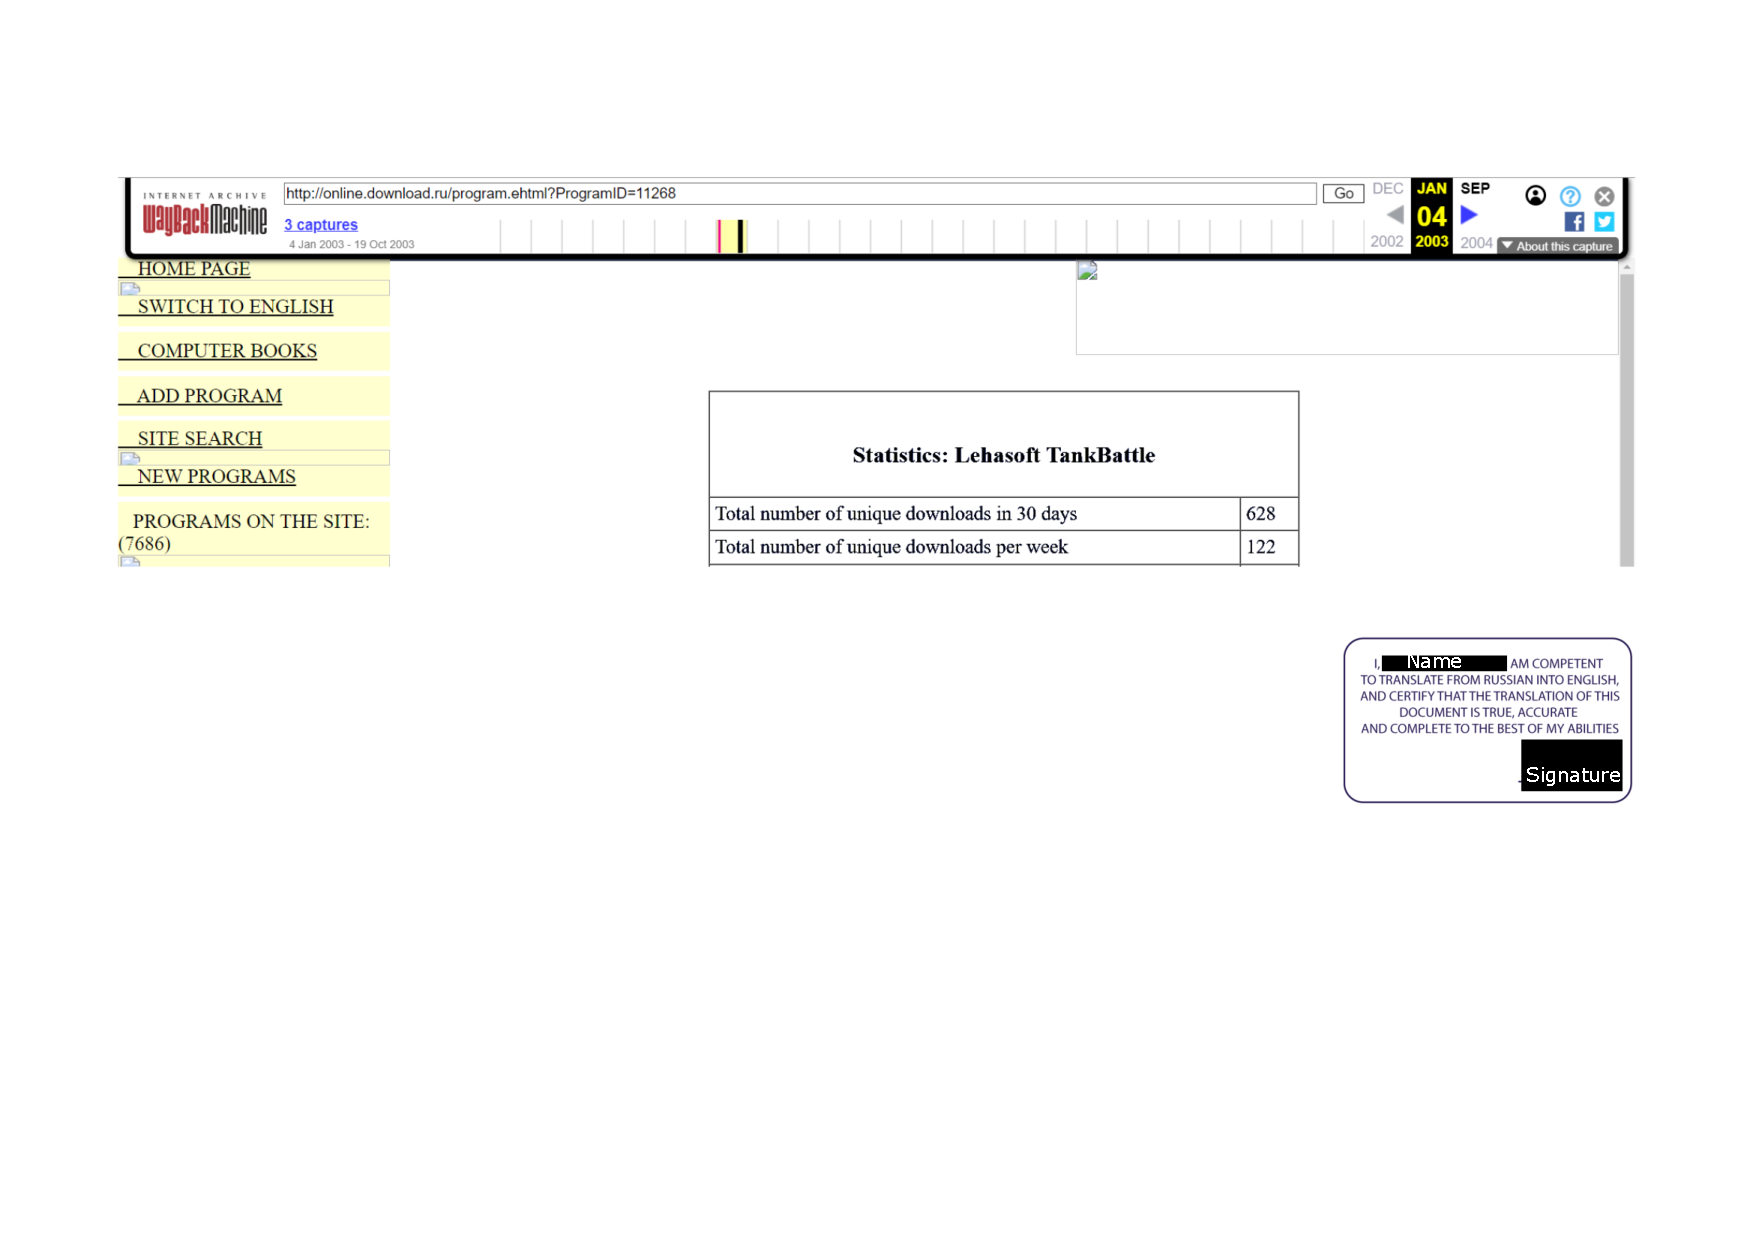
\includepdf[pages=-,angle=90]{tankbattle-downloads_eng_ai_public}
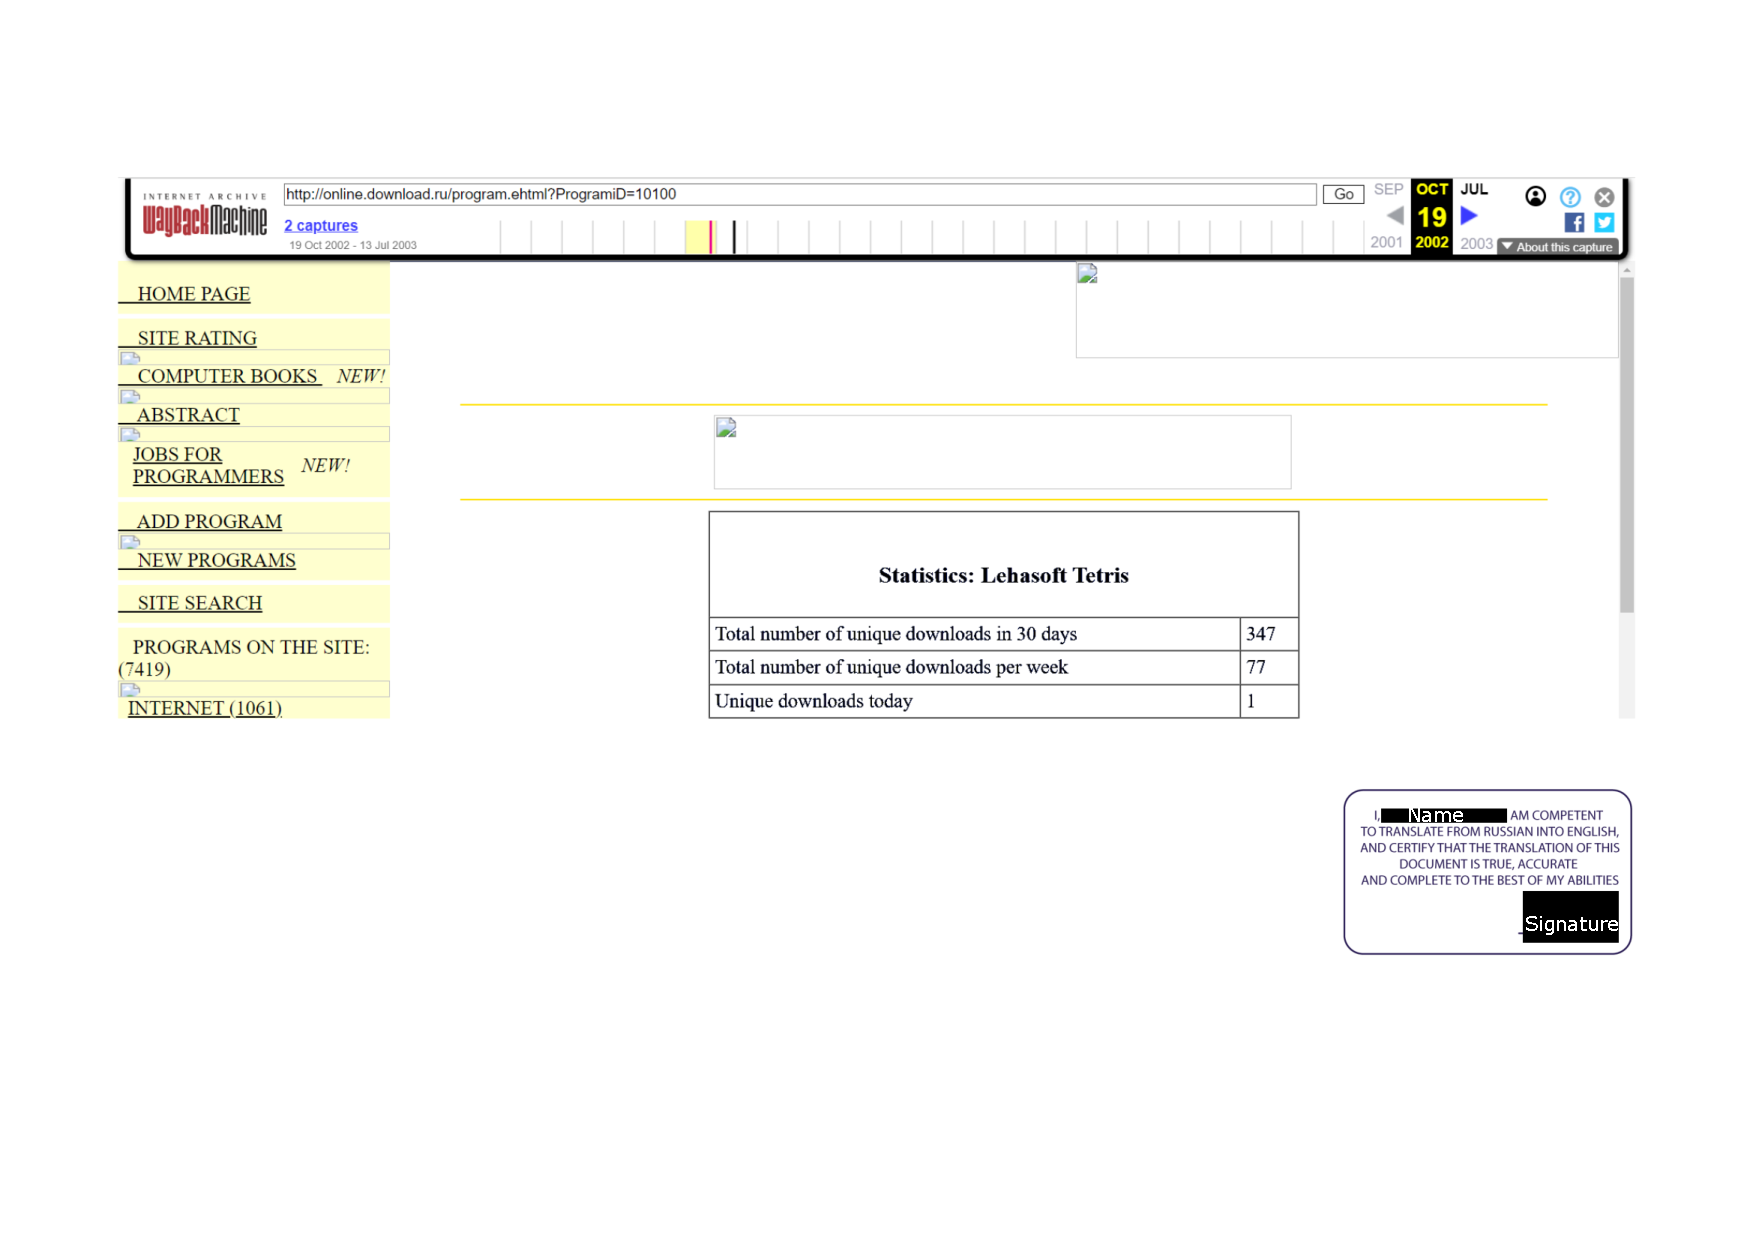
\includepdf[pages=-,angle=90]{tetris-downloads_eng_ai_public}
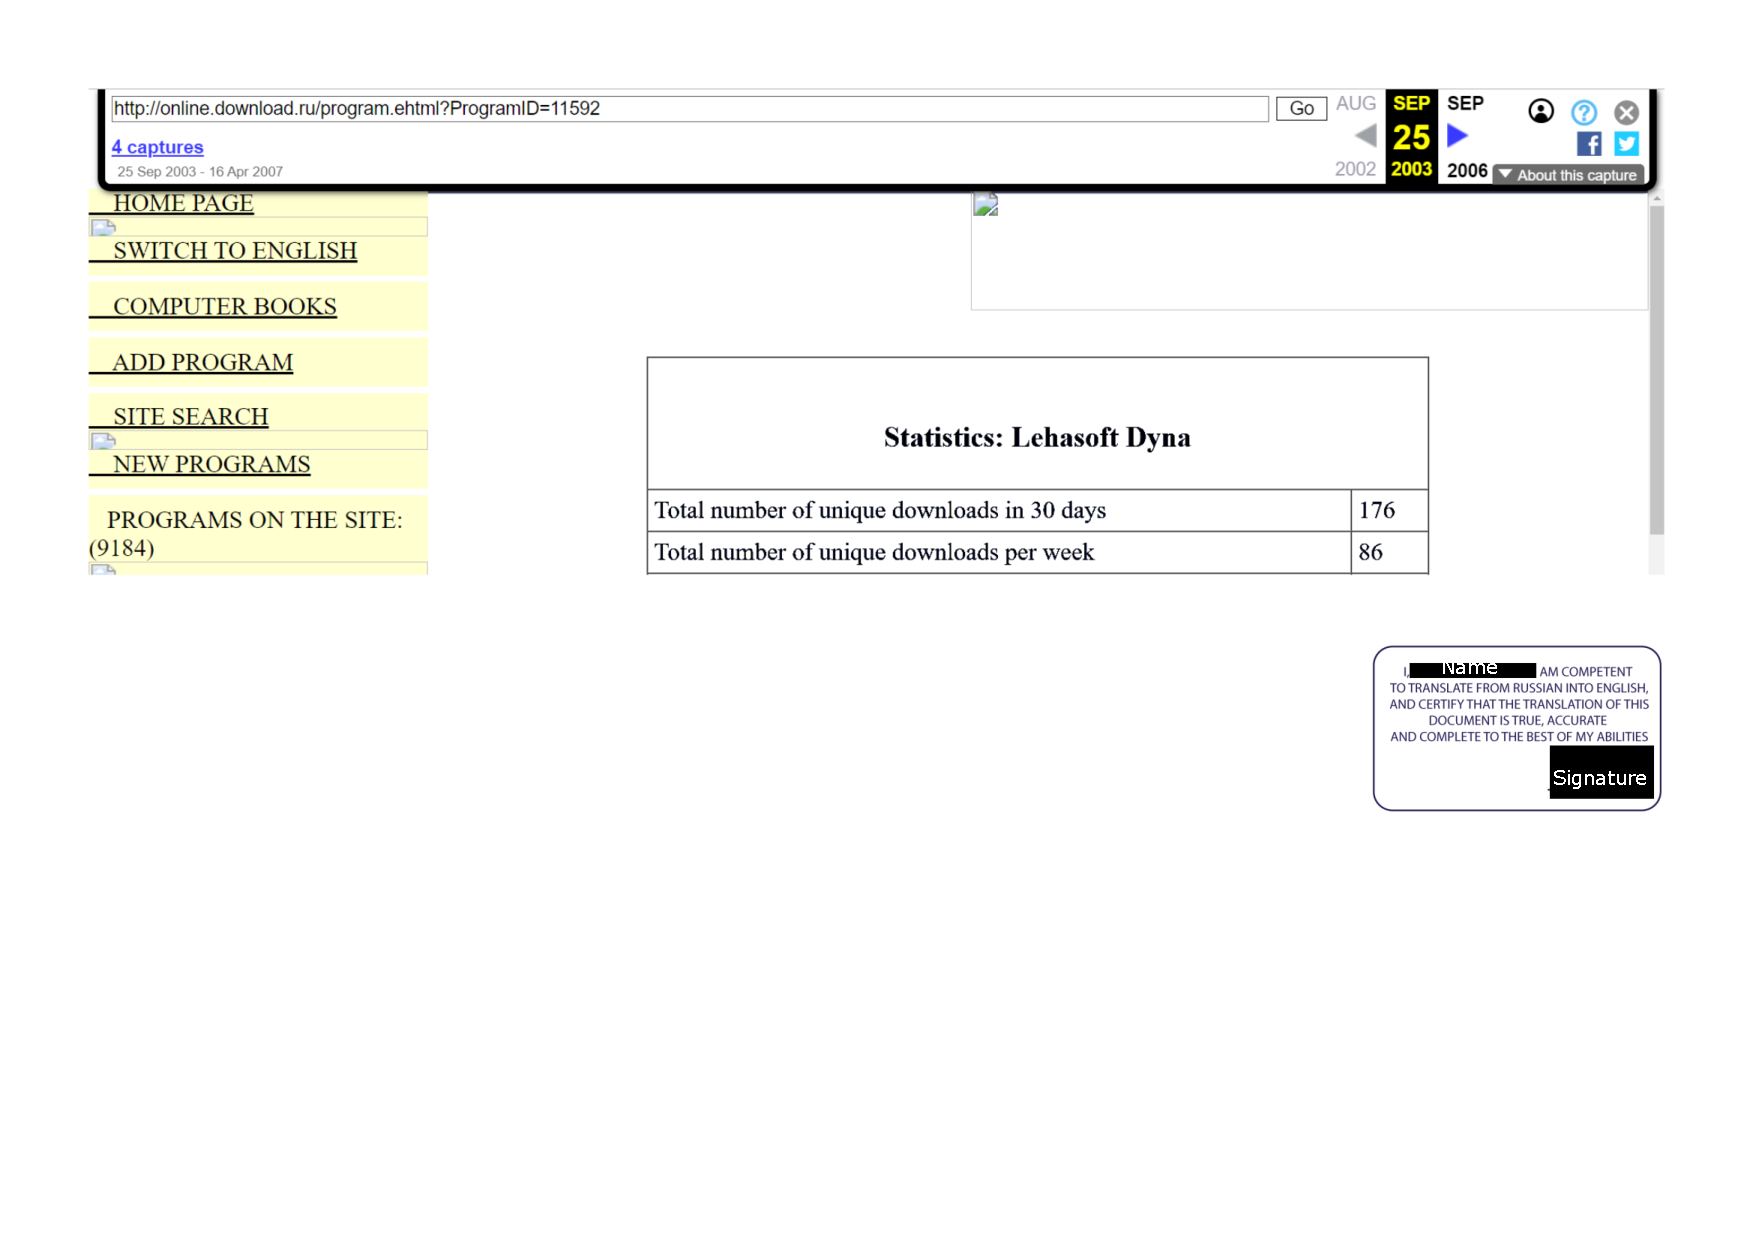
\includepdf[pages=-,angle=90]{dyna-downloads_eng_ai_public}

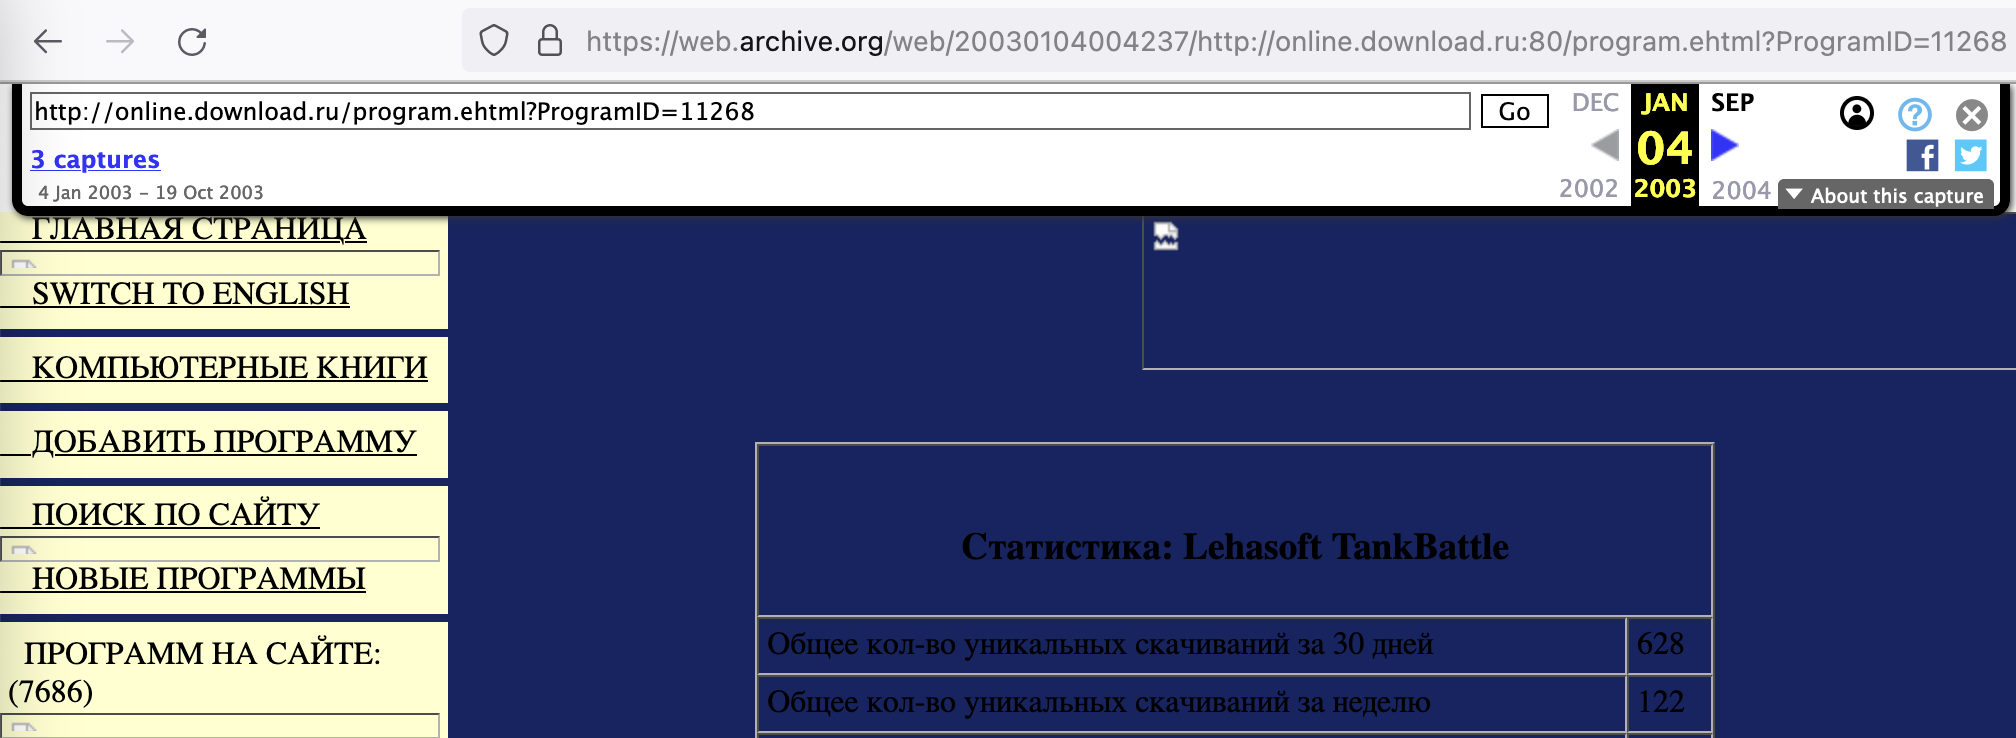
\includegraphics[width=40em]{tankbattle-downloads}

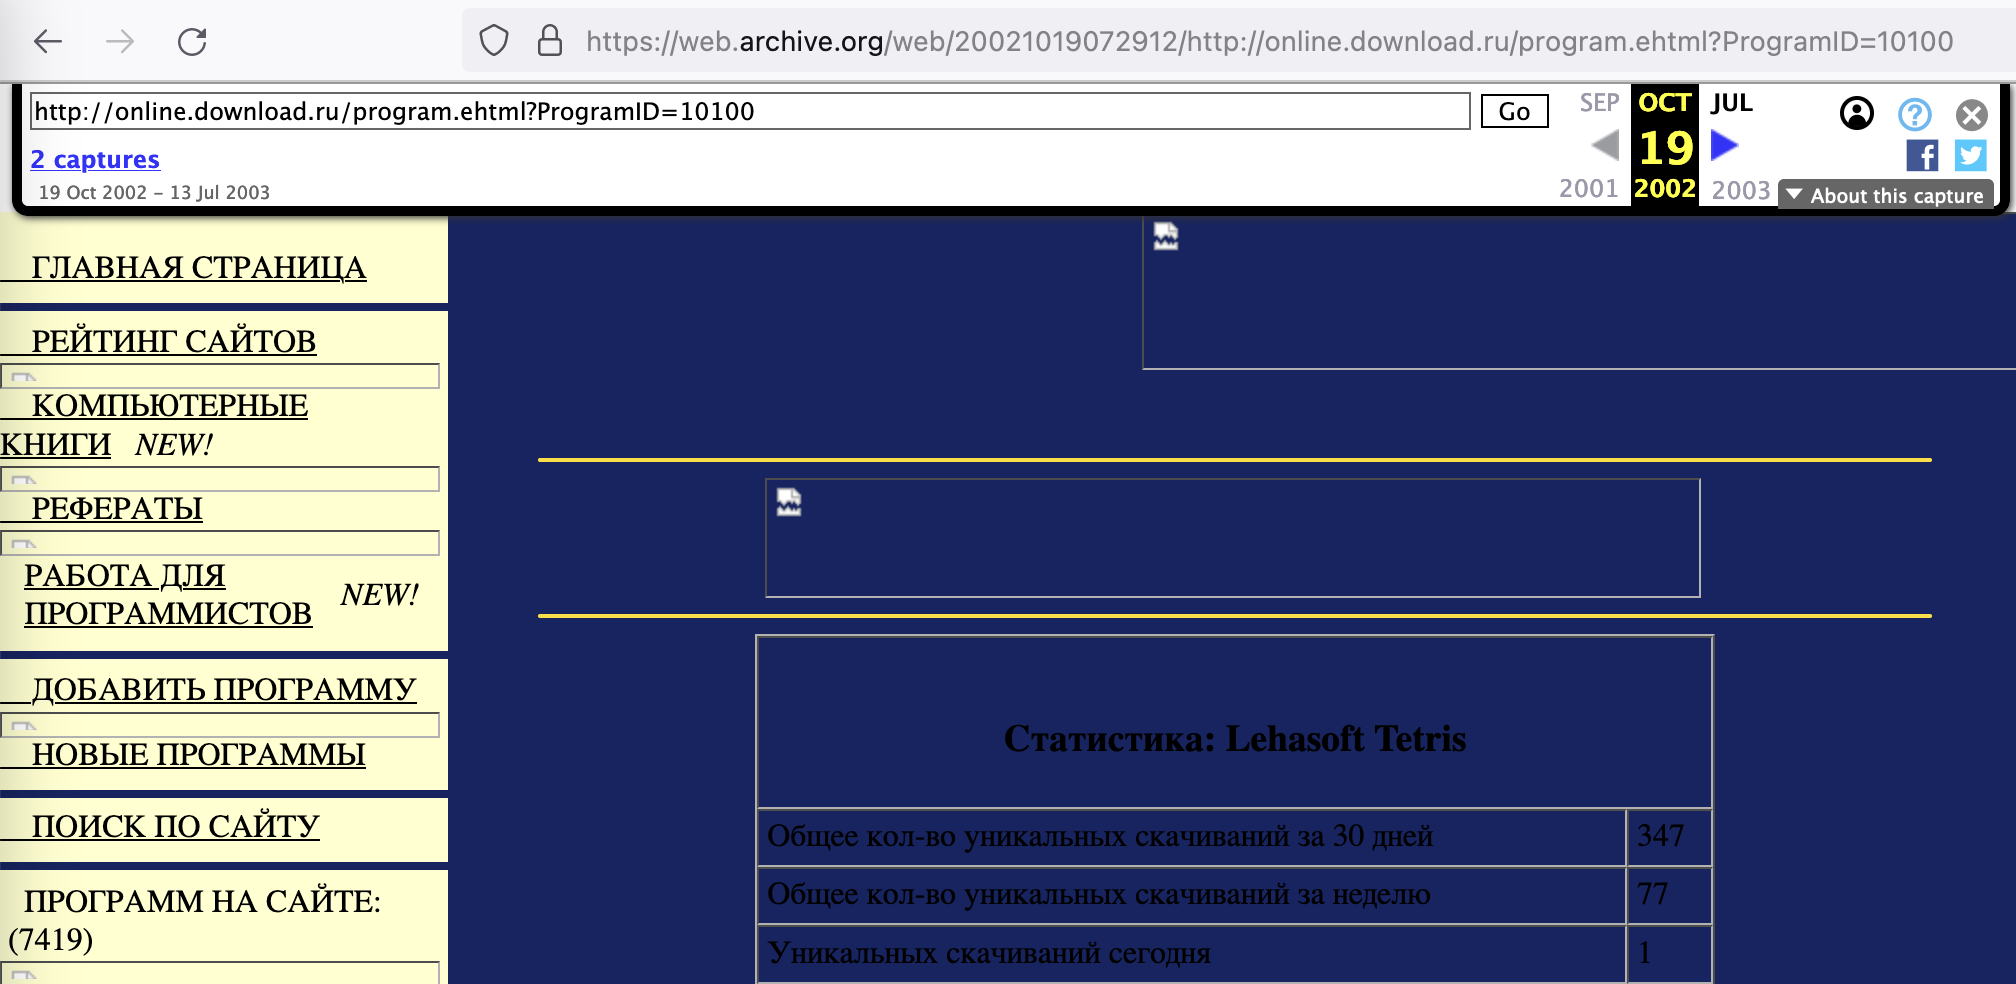
\includegraphics[width=40em]{tetris-downloads}

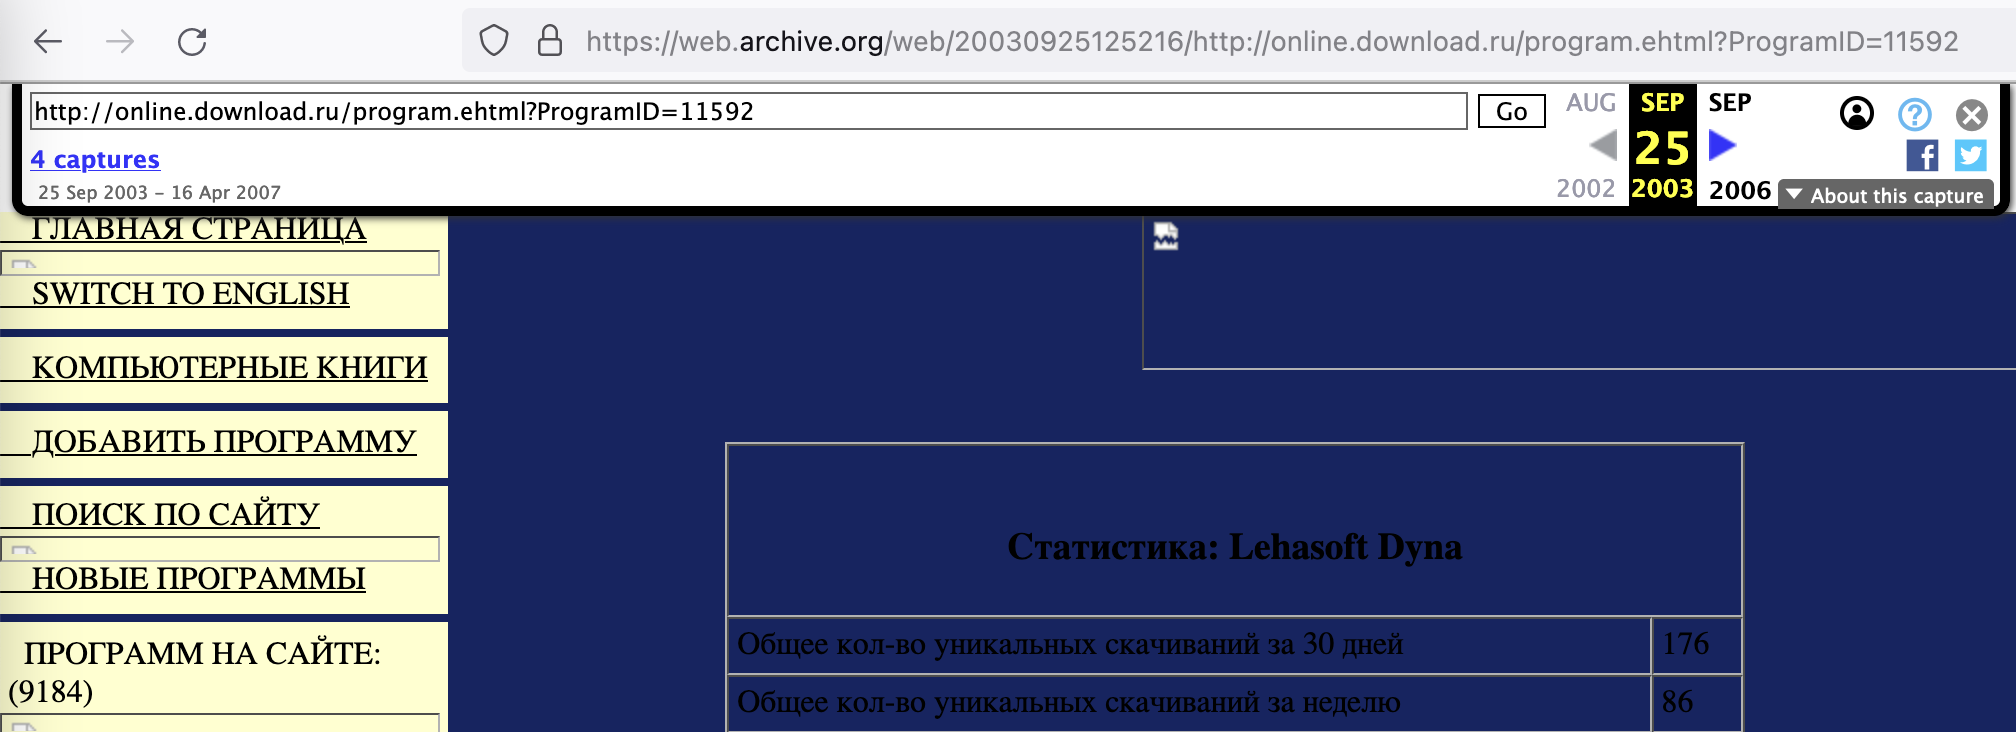
\includegraphics[width=40em]{dyna-downloads}

Эти игры публиковались под названием `Lehasoft'
(`Leha' неформальный вариант `Alexey' в России),
которое Алексей Инкин использовал тогда.
Его авторство подтверждается архивной версией его сайта 2002 года:

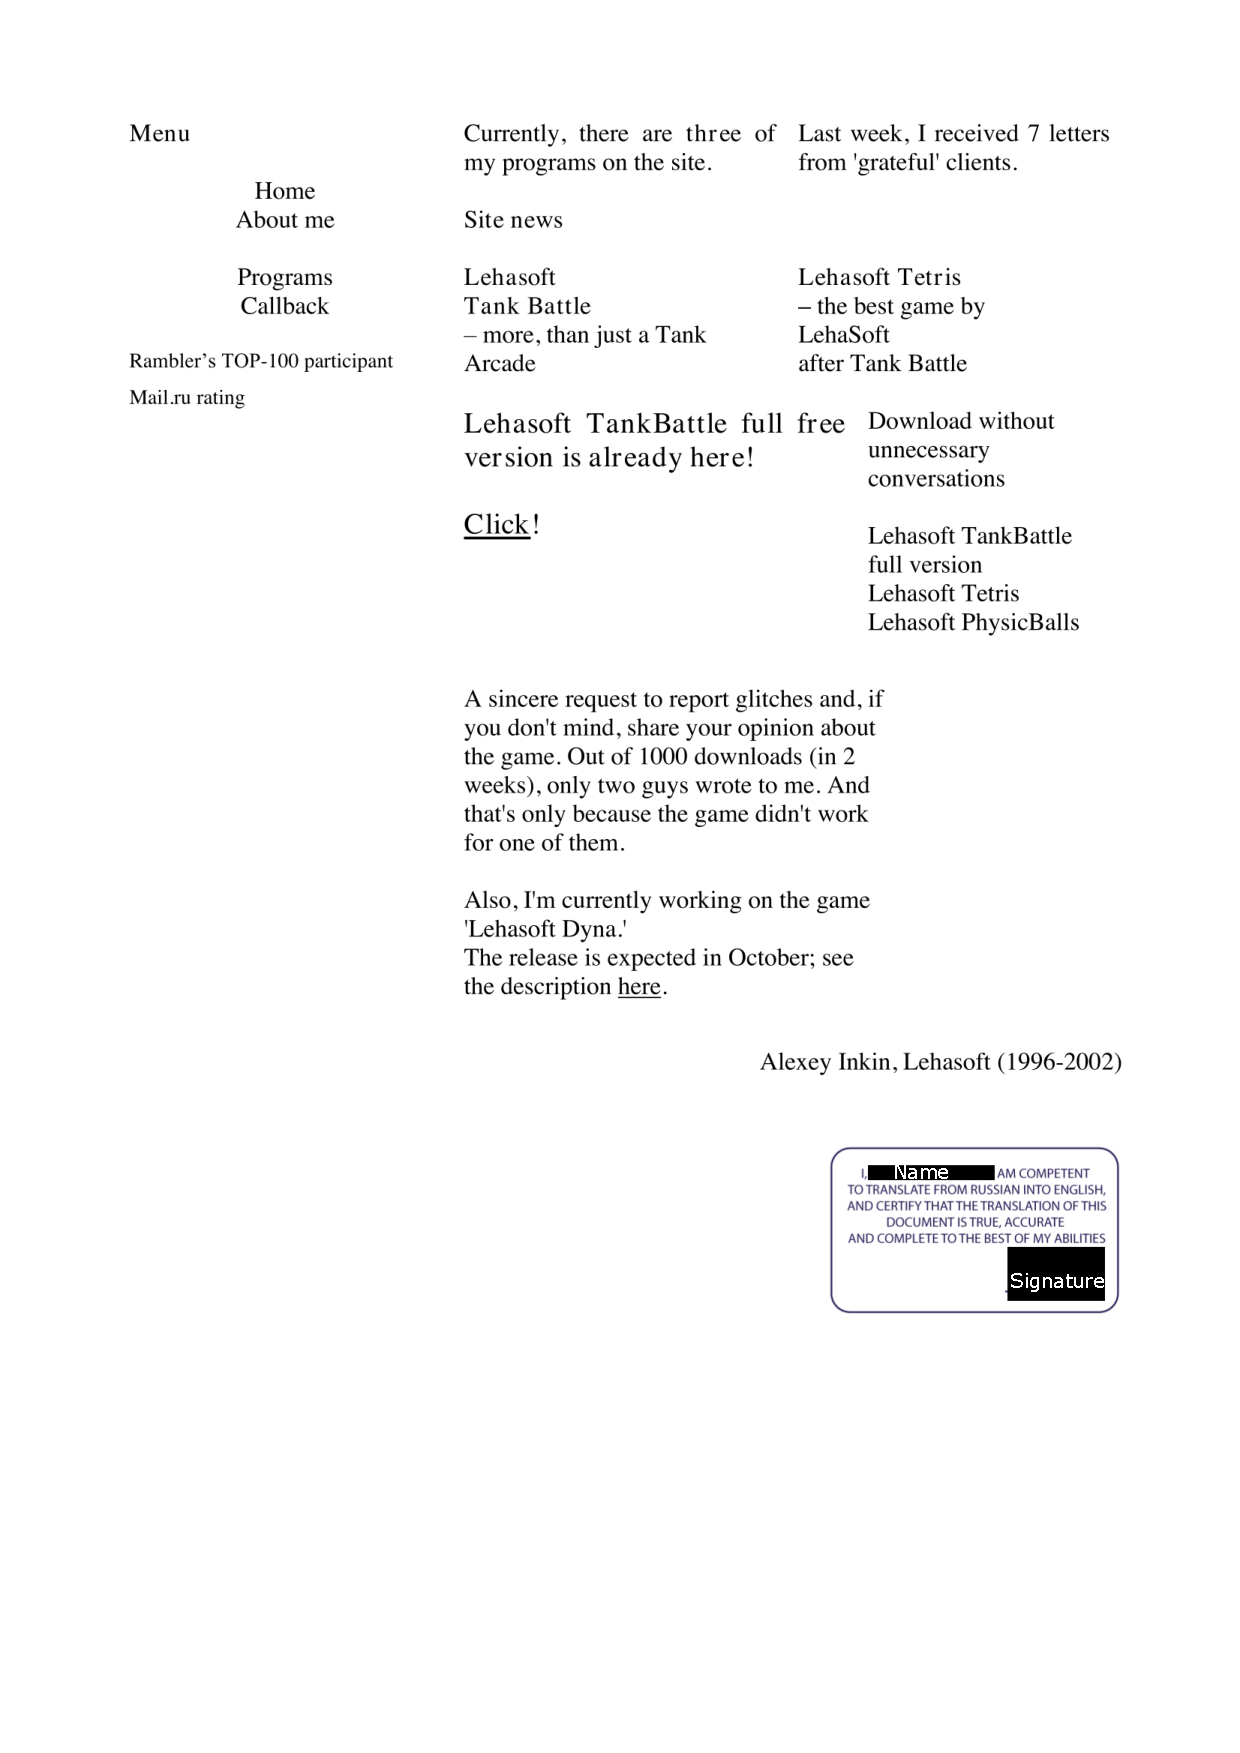
\includepdf[pages=-]{lehasoft-hotbox_eng_public}

\begin{center}
    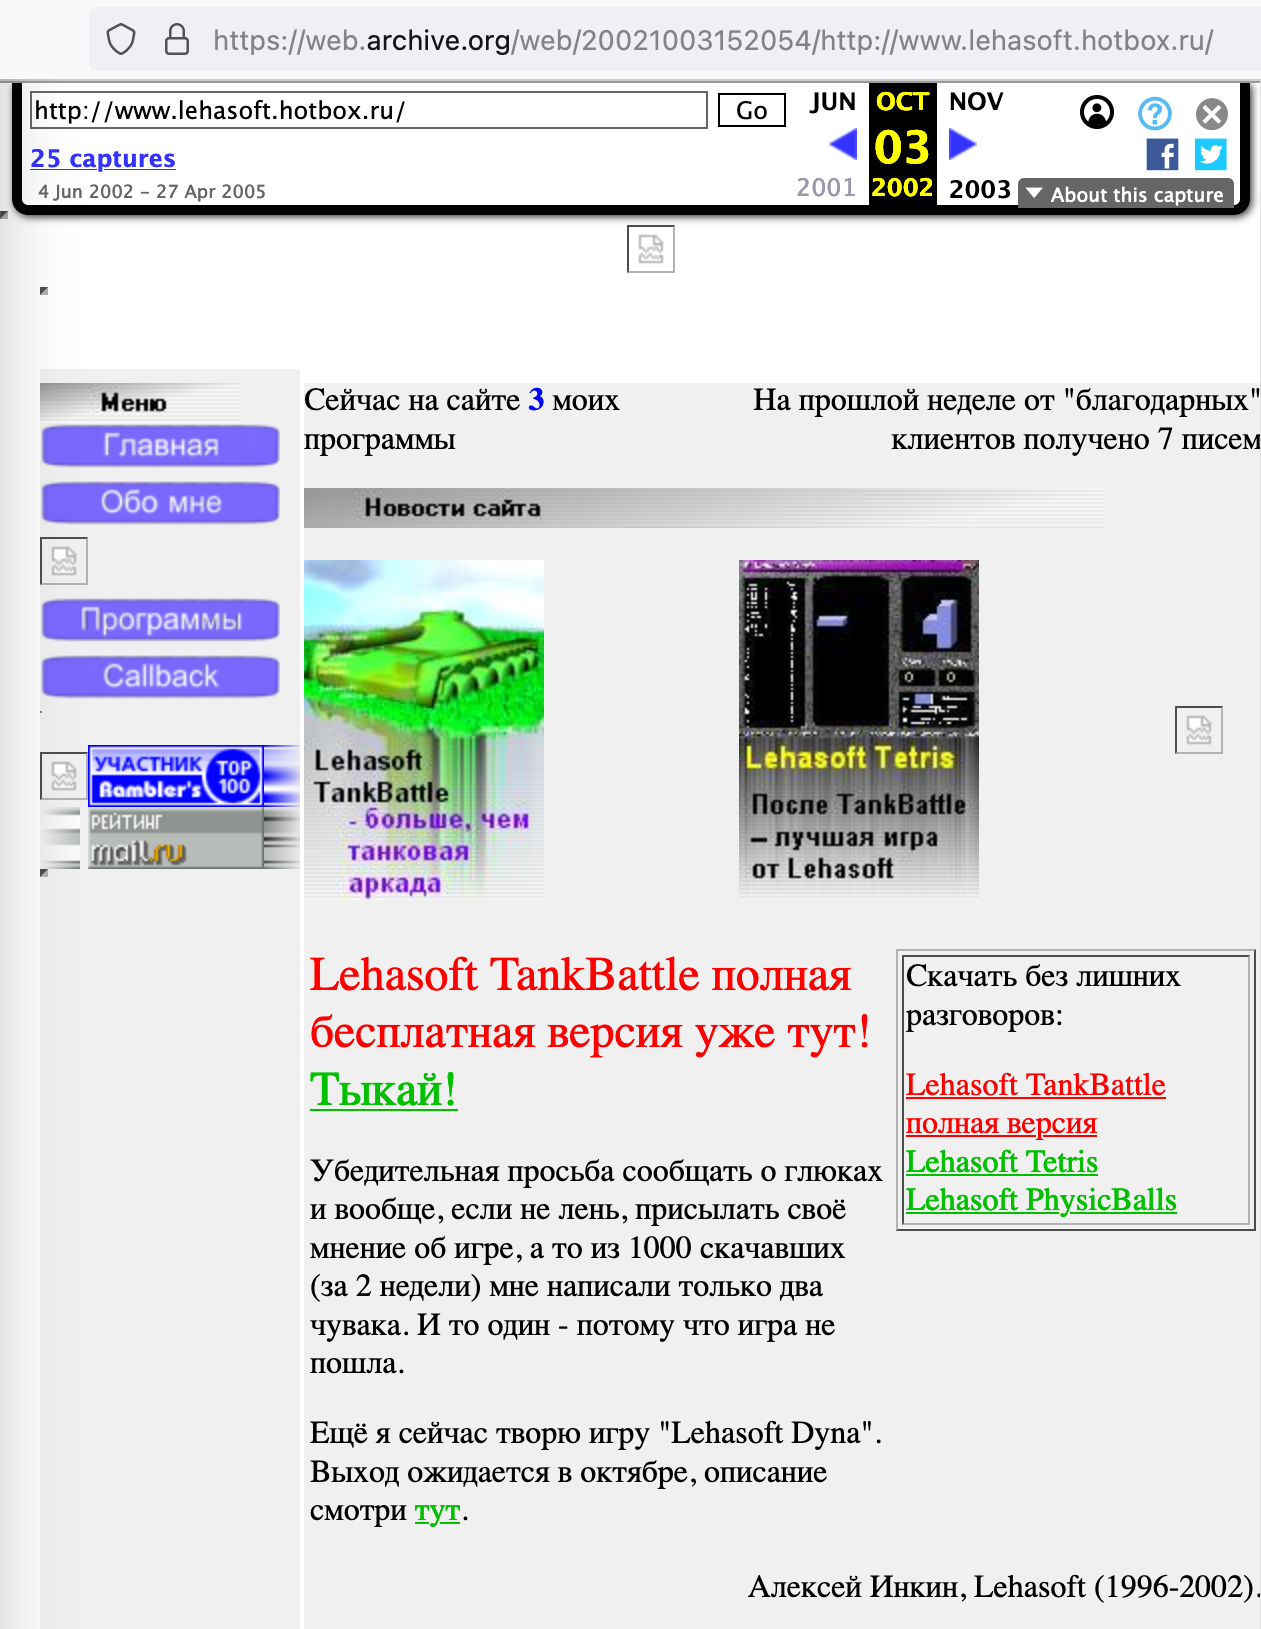
\includegraphics[width=\textwidth]{lehasoft-hotbox}
\end{center}

\pagebreak
